\section{Finding Top-k Teams}
\label{sec-tsimAlg}


\begin{figure}[tb!]
	%\vspace{-1ex}
	\begin{center}
		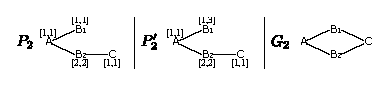
\includegraphics[scale=1.38]{./fig/consistency_motivation.eps}
	\end{center}
	\vspace{-3ex}
	\caption{Pattern satisfiability}
	\vspace{-4ex}
	\label{fig-consistency-example}
\end{figure}

In this section, we first study the pattern satisfiability problem for team formation, then introduce two optimization techniques, and finally we present our  batch algorithm for top-$k$ team formation.

% with one novel feature and two optimizations, \ie pattern satisfiability check, and incremental computing for radius varied balls and density based filtering optimization, compared with traditional algorithms for \warn{strong simulation}~\cite{MaCFHW14}.


\subsection{Pattern Satisfiability}
Different from graph simulation \cite{infsimu95} and its extensions \cite{FanLMTWW10,MaCFHW14},
there exist patterns that cannot match any data graph via team simulation, due to the presence of capacity constraints on patterns. We illustrate this with an example.
%\looseness=-1

\begin{example}
\label{exm-consistency}
\ni(1) For pattern $P_2$ in Fig.~\ref{fig-consistency-example},
one can verify that there exist no data graphs $G$ such that $P_2 \eeps G$ because (a) for any nodes $v$ in $G$, if $v$ matches with the node labeled with $B_2$, then it must match with the node labeled with $B_1$, and, hence, (b) the capacity upper bound on $B_1$ should not be less than the lower bound on $B_2$.

\sstab(2) However, pattern $P'_2$ in Fig.~\ref{fig-consistency-example} is satisfiable as $P'_2 \eeps G_2$, and pattern $P_1$ in Fig.~\ref{exm-motivation} is also satisfiable as $P_1 \eeps G_1$.
\end{example}


%Given a pattern $P$, \grouprec firstly checks whether $P$ is satisfiable.

We say that a pattern $P$ is {\em satisfiable} iff there exists a data graph $G$ such that $P$ matches $G$ via team simulation, \ie $P \eeps G$.
The good news is that checking the satisfiability of pattern graphs can be done in low polynomial time.

\begin{prop}
\label{prop-pattern-consistency}
The satisfiability of patterns $P$ can be checked in $O(|P|^2)$ time.
\end{prop}

By treating $P$ as both data and pattern graphs, compute the maximum match relation $M$ in $P$ for $P$, via graph simulation.
Then pattern $P$ is satisfiable iff for each $(u, v)\in M$ with the capacity bounds $[x_u, y_u]$ on $u$ and $[x_v, y_v]$ on $v$, respectively, $x_v \leq y_u$ holds. Observe that the size of $M$ is bounded by $|P|^2$, and pattern graphs are typically small.

By Proposition~\ref{prop-pattern-consistency}, we shall consider  satisfiable pattern graphs only  in the sequel.


\eat{%%%170721
Pattern graphs are typically small, and we only consider  satisfiable patterns in the sequel, by Proposition~\ref{prop-pattern-consistency}.
}%%%170721

\subsection{Batch Algorithm}

We then introduce two techniques for optimizing the computation of team simulation.

\stitle{Handling radius varied balls}. \teamF{} is to find top-$k$ teams within balls $\ball{[v, t]}$, where $v \in V$ and $t \in [1,r]$.
%centered at each node in $G$ with radius $t$ varying from 1 to $r$.
However, it is very costly to construct all $r|V|$ balls, and to compute perfect subgraphs in all of them.
Indeed it is also not necessary, and it only needs to construct and compute the matches for a number of $|V|$ balls, \ie the set of balls $\ball{[v, r]}$
where $v \in V$ and radius is $r$, and then incrementally computes the perfect subgraphs for balls $\ball{[v, t]}$ ($t \in [1,r-1]$) from the match graphs for ball $\ball{[v, r]}$, as shown below.

\vspace{-1ex}
\begin{theorem}
	\label{thm-tsim-radius}
	Given $P$, ball $\ball{[v, r]}$ and $\ball{[v, t]}$ ($t \in[1,$ $r-1]$) in $G$,
	(1) if $P\eps \ball{[v, t]}$, then $P\eps \ball{[v, r]}$; and
	(2) if $G_s$ (resp. $G'_s$) is the match graph \wrt the maximum match relation $M$ (resp. $M'$) in $\ball{[v, r]}$ (resp. $\ball{[v, t]}$) for $P$ via graph simulation, then $M' \subset M$, and $G'_s$ is a subgraph of $G_s$.	
\end{theorem}
\looseness=-1

When we have the match graph $G_s$ in $\ball{[v, r]}$ for $P$ via graph simulation, to compute the perfect subgraph in $\ball{[v, t]}$ ($t \in [1,r-1]$) for $P$ via team simulation, we need to
(1) first identify the subgraph $G_s^{t}$ in $G_s$ belonging to $\ball{[v, t]}$, which can be easily identified in the process for constructing $\ball{[v, r]}$ without extra computation;
(2) check whether $G_s^{t}$ is already a match graph for $P$ in $\ball{[v, t]}$ via graph simulation; if not, remove the unmatched nodes and edges from $G_s^{t}$ until find the match graph $G'_s$ for $P$ in $\ball{[v, t]}$. This can be achieved by executing an efficient incremental process in~\cite{FanWW13-tods}; and
(3) finally check whether capacity bounds are satisfied. If so, $G'_s$ is the perfect subgraph in $\ball{[v, r]}$ for $P$ via team simulation.

\stitle{Density based ball filtering}. We further reduce the number of balls to speedup the process by adopting the density based filtering technique.
The key idea is to tell whether a ball is possible to produce one of the final top-$k$ matches.

Given a ball $\ball{[v,r]}$, we compute the density upper bound  $\density{\hat{G}_s}$,
where $\hat{G}_s$ is a subgraph of $\ball{[v,r]}$.
If the bound is larger than the density of the current $k$-th result, \ie there is a possibility for the ball;
Otherwise, the ball is simply ignored to avoid redundant computations.

The trick part is how to efficiently compute the upper bound of $\density{\hat{G}_s}$ for each ball in $G$.
As the best densest subgraph algorithms are in $O(|\ball{[v,r]}|^3)$ time \cite{maximumDenseSubgraph}, which is costly,
we utilize an important result in~\cite{EVMK12}, shown below.



\begin{lemma}
	\label{lemma-approximation-bound}
	Let $\density{H_{c}}$ and $\density{H_{d}}$ be the density of the maximum core  $H_{C}$  and the  densest subgraph $H_{d}$ of graph $H$. Then (1) $\density{H_{c}}\leq \density{H_{d}} \leq 2*\density{H_{c}}$; and (2) there exists an algorithm that computes $\density{H_{c}}$ in $O(|E_H|)$ time~\cite{EVMK12}.
\end{lemma}


Here the maximum core $H_{C}$ of a graph $H$ is a subgraph of $H$ whose node degree is at least $\rho$, where $\rho$ is the maximum possible one. By Lemma~\ref{lemma-approximation-bound}, we use $2*\density{H_{c}}$ as the density upper bound for filtering unnecessary balls.


We are now ready to present our batch algorithm for \teamF{}.

\stitle{Algorithm \grouprec.} As shown in Fig.~\ref{alg-grouprec}, it takes input as $P$, $G$, and two integers $r$ and $k$, and outputs the top-$k$ densest perfect subgraphs in $G$ for $P$.
It firstly checks whether $P$ is satisfiable (line 1).
If so, for each ball $\ball{[v,r]}$ in $G$, it computes the maximum core $\ball{}_{C}$ of $\ball{[v,r]}$, and checks whether the
density based ball filtering condition holds (lines 3-6).
If so, it skips the current ball, and moves to the next one;
otherwise, it computes the perfect subgraph $G_{s}$ of $P$ in $\ball{[v,r]}$ via team simulation by invoking \rgraphsim (line 7, see full version~\cite{fullvldb18}),
an adaption from graph simulation~\cite{infsimu95,FanLMTWW10} and checking capacity bounds (line 8).
It then computes perfect subgraphs $G'_{s}$ of $P$ in inner balls $\ball{[v,t]}$ by invoking \incsim, an extension of the data incremental algorithms in \cite{FanWW13-tods} and checking capacity bounds (lines 9-11).
%Procedure \rgraphsim is deferred to the appendix, which is an adaption from graph simulation~\cite{infsimu95,FanLMTWW10}.}
%by extending from directed to undirected graphs,  incorporating the capacity constraint check, and only maintaining the capacity bounds satisfied perfect subgraphs.

\stitle{Correctness \& complexity analyses}. The correctness of \grouprec is assured by the following.
%(1) There is a unique perfect subgraph in each ball of $G$.

\sstab(1) The correctness of \rgraphsim (resp. \incsim) can be verified along the same lines as graph simulation~\cite{infsimu95} (resp. incremental simulation \cite{FanWW13-tods}).

\sstab(2) Theorem~\ref{thm-tsim-radius} and Lemma~\ref{lemma-approximation-bound}.
It takes $O(|P|^2)$ to check pattern satisfiability, $O(|V||P||G|)$ to compute team simulation, $O(r|V||V_{P}||E|)$ to incrementally compute matches in inner balls, and $O(|V||E|)$  to compute the density of the maximum core for $|V|$ balls.
Thus \grouprec is in $O(|P|^2+|V||P||G|+r|V||V_{P}||E|)$. However, actual time is much less due to density based ball filtering and that  $O(r|V||V_{P}||E|)$ is the worst case complexity for incremental process, while $r$ is small, \ie 2 or 3.



\begin{figure}[t!]
	%\vspace{-2ex}
	\begin{center}
		{\small
			\myhrule
			\vspace{-3ex}
			\mat{0ex}{
				\sstab {\sl Input:\/} $G(V$, $E)$, $P(V_P$, $E_P)$, and positive integers $r$ and $r$.\\
				{\sl Output:\/} Top-$k$ densest teams.\\
				\sstab \bcc \hspace{1ex}\= \If $P$ is unsatisfiable \Then \Return $nil$;\\
				\icc \> $L_{k} := \emptyset$;\\
				\icc \> \For each ball $\ball{[v,r]}$ in $G$ \Do\\
				\icc \>\hspace{2ex}\= compute the maximum core $\ball{}_{C}$ of the ball $\ball{[v,r]}$;\\
				\icc \>\> \If 2*$\density{\ball{}_C} <$  the density of the $k$-th result in $L_{k}$ \Then\\
				\icc  \>\>\hspace{2ex}\= \Continue;\\
				\icc \>\> $G_s$ := \rgraphsim$(P, \ball{[v,r]})$; \\
				\icc \>\> If $G_s$ satisfy capacity bounds on $P$ \Then Insert $G_s$ into $L_{k}$;\\
				\icc \>\> \For each ball $\ball{[v,t]}$ with $t\in[1,r-1]$ \Do\\
				\icc \>\>\hspace{2ex}\= $G'_s$ := \kw{incSim}$(G_s, P, \ball{[v,t]})$;\\
				\icc \>\>\> If $G'_s$ satisfy capacity bounds on $P$ \Then Insert $G'_s$ into $L_{k}$;\\
				%\icc \>\> \If $\density{G_s}>$ the density of the $k$-th result in $L_{k}$ \Then\\
				%\icc \>\> \If $\density{G_s}>$ the density of $kth$ result in $L_{k}$ and there exists\\
				%     \>\>\hspace{0.5ex}   no $G'_s$ in $L_{k}$ that is same with $G_{s}$ \Then\\
				%\icc \>\>\hspace{2ex}\= remove the $k$-th result in $L_{k}$ and insert $G_s$ into $L_{k}$;\\
				\icc \>\, \Return $L_{k}[0:k-1]$.
			}
			
			\vspace{-4ex} \myhrule
		}
	\end{center}
	\vspace{-3ex}
	\caption{Algorithm \grouprec}
	\label{alg-grouprec}
	\vspace{-3ex}
\end{figure}

